\documentclass[]{article}
\usepackage{lmodern}
\usepackage{natbib}
\usepackage[figuresright]{rotating}
\usepackage{amsmath,amssymb}
\usepackage{bbm}
%\usepackage{subfigure}
\usepackage{graphicx}
\usepackage{subcaption}
\captionsetup{compatibility=false}
\font\myfont=cmr12 at 15pt
\renewcommand{\baselinestretch}{1.0}
\setlength{\baselineskip}{20pt}
\usepackage{amssymb,amsmath}
\usepackage{ifxetex,ifluatex}
\usepackage{}
\linespread{1.6} 
\usepackage{fixltx2e} % provides \textsubscript
\ifnum 0\ifxetex 1\fi\ifluatex 1\fi=0 % if pdftex
  \usepackage[T1]{fontenc}
  \usepackage[utf8]{inputenc}
\else % if luatex or xelatex
  \ifxetex
    \usepackage{mathspec}
  \else
    \usepackage{fontspec}
  \fi
  \defaultfontfeatures{Ligatures=TeX,Scale=MatchLowercase}
\fi
% use upquote if available, for straight quotes in verbatim environments
\IfFileExists{upquote.sty}{\usepackage{upquote}}{}
% use microtype if available
\IfFileExists{microtype.sty}{%
\usepackage{microtype}
\UseMicrotypeSet[protrusion]{basicmath} % disable protrusion for tt fonts
}{}
\usepackage[margin=1in]{geometry}
\usepackage{hyperref}
\urlstyle{same}  % don't use monospace font for urls
\usepackage{graphicx,grffile}
\makeatletter
\def\maxwidth{\ifdim\Gin@nat@width>\linewidth\linewidth\else\Gin@nat@width\fi}
\def\maxheight{\ifdim\Gin@nat@height>\textheight\textheight\else\Gin@nat@height\fi}
\makeatother
% Scale images if necessary, so that they will not overflow the page
% margins by default, and it is still possible to overwrite the defaults
% using explicit options in \includegraphics[width, height, ...]{}
\setkeys{Gin}{width=\maxwidth,height=\maxheight,keepaspectratio}
\IfFileExists{parskip.sty}{%
\usepackage{parskip}
}{% else
\setlength{\parindent}{0pt}
\setlength{\parskip}{6pt plus 2pt minus 1pt}
}
\setlength{\emergencystretch}{3em}  % prevent overfull lines
\providecommand{\tightlist}{%
  \setlength{\itemsep}{0pt}\setlength{\parskip}{0pt}}
\setcounter{secnumdepth}{5}
% Redefines (sub)paragraphs to behave more like sections
\ifx\paragraph\undefined\else
\let\oldparagraph\paragraph
\renewcommand{\paragraph}[1]{\oldparagraph{#1}\mbox{}}
\fi
\ifx\subparagraph\undefined\else
\let\oldsubparagraph\subparagraph
\renewcommand{\subparagraph}[1]{\oldsubparagraph{#1}\mbox{}}
\fi

%%% Use protect on footnotes to avoid problems with footnotes in titles
\let\rmarkdownfootnote\footnote%
\def\footnote{\protect\rmarkdownfootnote}

%%% Change title format to be more compact
\usepackage{titling}
\usepackage{inputenc}
\usepackage[english]{babel}

\setlength{\parindent}{2em}
\setlength{\parskip}{1em}

% Create subtitle command for use in maketitle
\providecommand{\subtitle}[1]{
  \posttitle{
    \begin{center}\large#1\end{center}
    }
}



\setlength{\droptitle}{-2em}
 \title{{\myfont Bayesian Inference for Cox Proportional Hazard Models with Partial Likelihoods, Semi-Parametric Covariate Effects and Correlated Observations}}
    \pretitle{\vspace{\droptitle}\centering\huge}
  \posttitle{\par}
    \preauthor{\centering\large\emph}
  \postauthor{\par}
      \predate{\centering\large\emph}
  \postdate{\par}
    \date{07/02/2020}


\begin{document}
	
\maketitle

\begin{abstract}
We develop an approximate Bayesian inference methodology for the Cox Proportional Hazards model for survival data with partial likelihood, semi-parametric covariate effects and correlated survival times. Bayesian inference provides model-based uncertainty quantification of the smoothness parameters and between-group standard deviations. The use of partial likelihood avoids smoothness assumptions on the baseline hazard, leading to improved inferences over current methods for approximate Bayesian inference for this model (INLA). A simulation study demonstrates the superior accuracy of our approximations over existing methods when the baseline hazard is not smooth. Analysis of two benchmark datasets demonstrates the improved accuracy of our method over INLA when compared to the frequentist generalized additive models (GAMs), but in contrast to GAMs, we yield full posterior uncertainty for the smoothness of the semi-parametric effect and the between-subject standard deviation. An R package implementing our method will be released publicly.
\end{abstract}


\section{Introduction}
Survival data consists of times to an event of interest such as mortality or morbidity.  When analysing survival data, the Cox proportional hazards (Cox PH) model is a common choice. The Cox PH model assumes that any two subjects' event hazards are proportional as a function of time, with the ratio depending on covariate effects which are modelled as unknown linear or smooth functions and inferred from the observed data. Event times may be correlated within the sample, for example when the response is time to kidney failure for the left and right kidneys from the same subject. In order to avoid having to make assumptions about the shape of the unknown common baseline event hazard, a partial likelihood is often used, which does not depend on this quantity. The use of Bayesian inference with the Cox PH model is desirable as this yields model-based estimation and uncertainty quantification for the smoothness of the covariate effects, and in the case of correlated survival times, the between-group standard deviations. However, existing methods for approximate Bayesian inference based on Integrated Nested Laplace Approximations (INLA) \citet{inla} cannot be applied to the Cox PH model with partial likelihood, and hence require restrictive smoothness assumptions to be made about the baseline hazard.

Recently, \citet{casecross} developed an approximate Bayesian inference methodology for a model involving a partial likelihood. Their methodology includes smooth covariate effects and yields full posterior uncertainty for the smoothness parameters, an improvement over existing frequentist methods based on Generalized Additive Models (GAMs), and they demonstrate up to an order of magnitude improvement in computation time when compared to sampling-based approaches to Bayesian inference. They note in their discussion that the partial likelihood involved in the Cox PH model has a similar form to the partial likelihood from their model, and that the Cox PH model with partial likelihood would be a feasible extension of their work.

In this paper we extend the approximate Bayesian inference methodology of \citet{casecross} to the Cox proportional hazard models with partial likelihood. Our methodology accommodates semi-parametric smoothing effects and correlation between observed survival times. We demonstrate improved accuracy over INLA in simulations and two data analysis examples, and provide model-based estimation and uncertainty quantification for the smoothness of effects and between-subject standard deviations.

The remainder of this paper is organized as follows. In \S\ref{sec:prelim}, we describe the Cox proportional hazard model and the partial likelihood function, and review the approximate Bayesian inference methodology of \citet{casecross}. In \S\ref{sec:method}, we describe our proposed methodology. In \S\ref{sec:example} we illustrate our methodology in a simulation study and through the analysis of two benchmark datasets. We conclude in \S\ref{sec:discussion} with a discussion.



\section{Preliminaries}\label{sec:prelim}
\subsection{Cox Proportional Hazard Model}
Let T denote a random variable representing the time to some event, supported on the interval $[0,\infty)$. For $t\in[0,\infty)$ the \textit{hazard function} $h(t)$ of $T$ is defined as:
\begin{equation}\begin{aligned}\label{eqn:hazard}
h(t) = \lim_{s\to 0} \frac{P(t\le T \le t+s |T\ge t)}{s}
\end{aligned}\end{equation}
Suppose we observe $i = 1,\ldots,n$ groups each with $j = 1,\ldots,n_{i}$ survival times. For example, we may observe $n$ subjects with $n_{i}$ measurements per subject. Denote the random variable representing the $j^{th}$ survival time in the $i^{th}$ group by $Y_{ij}$, and denote the survival times by $y = \left\{y_{ij}: i = 1,\ldots,n; j = 1,\ldots,n_{i} \right\}$. When there are some survival data in a data-set that are not observed exactly, we call these observations $censored$. Right-censoring is a common case of censoring when some survival times are only known to be longer than some specific times. For example, if the observation $y_{ij}$ is right-censored, then the only information available for $Y_{ij}$ is that $Y_{ij} > y_{ij}$. We will focus on this type of censoring in this paper.
Define $h_{ij}(t)$ to be the hazard function for random variable $Y_{ij}$. The Cox PH model assumes \citep{coxph}
\begin{equation}\begin{aligned}\label{eqn:CoxHazardModel}
h_{ij}(t) = h_0(t)\text{exp}(\eta_{ij})
\end{aligned}\end{equation}
where $h_0(t)$ is an unknown baseline hazard function that does not depend on the covariates. The additive predictor $\eta = \left\{ \eta_{ij}: i = 1,\ldots,n; j = 1,\ldots,n_{i}\right\}$ links the covariates for observation $y_{ij}$ to the observed survival time:
\begin{equation}\begin{aligned}\label{eqn:eta}
\eta_{ij} =x_{ij}^{T}\beta+\sum_{q=1}^{r} \gamma_q(u_{q_{ij}}) +\xi_{i}
\end{aligned}\end{equation}
Here $x_{ij}$ is a $p$-dimensional vector of covariates that are modelled as having linear associations with the log-hazard, and $\beta = (\beta_{1},\ldots,\beta_{p})$ are regression coefficients. The $u_{q} = \left\{u_{qij}: i = 1,\ldots,n; j = 1,\ldots,n_{i} \right\}, q = 1,\ldots,r$ are covariate vectors whose association with the log-hazard is modelled non-parametrically through unknown smooth functions $\gamma_1,\ldots,\gamma_r$. The vector of group intercepts $\xi = \left\{ \xi_{i}: i=1,\ldots,n\right\}$, referred to as ``frailty'' coefficients in the context of survival analysis \citep{frailty}, are included to model correlation between survival times coming from the same group $i$.

Inference is carried out via a partial likelihood function. Define the \textit{risk set} $R_{ij} = \left\{k,l : y_{kl} \geq y_{ij}\right\}$, the set of  indices of survival times which occur at or after $y_{ij}$. For simplicity, assumes for each group $i$ observations $1,2,...,r_i$ are actually $observed$ distinct survival times and the rest $n_i - r_i$ observations are right-censored, then partial likelihood can be written as follows:
\begin{equation}\begin{aligned}\label{eqn:partial}
\pi(y|\eta) &= \prod_{i=1}^{n}\prod_{j=1}^{r_{i}} \bigg\{\frac{\exp[\eta_{ij}]}{{\sum_{l,k\in R_{ij}}^{}\exp[\eta_{lk}]}}\bigg \} \\
&= \prod_{i=1}^{n}\prod_{j=1}^{r_{i}} \bigg\{\frac{1}{{1 + \sum_{l,k\in R_{ij} , (l,k) \neq (i,j)}\exp[\Delta_{lk,ij}]}}\bigg \} \\
\end{aligned}\end{equation}
where $\Delta_{lk,ij} = \eta_{lk} - \eta_{ij}$. Note that $h_{0}(t)$ does not appear in the partial likelihood, and hence inference may be carried out in the absence of assumptions about $h_{0}(t)$. Also note that this partial likelihood can be written in the following form:
\begin{equation}\begin{aligned}\label{eqn:whyINLAfail1}
\pi(y|\eta) &= \prod_{i=1}^{n}\prod_{j=1}^{r_{i}} \pi(y_{ij}|\eta)
\end{aligned}\end{equation}
while in order for a model to be compatible with INLA, its likelihood must have the form:
\begin{equation}\begin{aligned}\label{eqn:whyINLAfail2}
\pi(y|\eta) &= \prod_{i=1}^{n}\prod_{j=1}^{n_{i}} \pi(y_{ji}|\eta_{ij})
\end{aligned}\end{equation}

\subsection{Approximate Bayesian Inference}

To perform Bayesian inference for this model, we specify prior distributions for the parameters. A joint Gaussian prior distribution with fixed covariance matrix is used for $\beta {\sim}  \text{N}(0,\Sigma_\beta)$; we follow \citet{casecross} and use $\Sigma_{\beta} = \sigma^{2}_{\beta}I_{p}$, with $\sigma^{2}_{\beta} = 1000$. The group intercepts are given independent Gaussian priors $\xi_{i} | \theta \stackrel{iid}{\sim} \text{N}(0,\sigma_{\xi}),i = 1,\ldots,n$ where $\sigma_{\xi}$ is the between-groups standard deviation. Let $U_{q} = \{U_{ql};l = 1, ...., m_q\}$ be the ordered vector of \textit{unique} values of covariate $u_q,q = 1,\ldots,r$; often these values are set by the user by discretizing the covariate $u_q$ into $m_q$ pre-specifed bins. To infer the infinite-dimensional parameters $\gamma_{q},q = 1,\ldots,r$, we approximate each by a piecewise constant function with jumps at the $U_{ql}$, which we denote as $\gamma(U_{ql}) = \Gamma_{ql}$. We define the vectors of function values $\Gamma_{q} = \left\{ \Gamma_{q1},\ldots,\Gamma_{qm_{q}}\right\}$ and these are given a joint Gaussian distribution $\Gamma_{q}|\theta\sim\text{N}\left[ 0,\Sigma_{q}(\sigma_{q})\right]$ which is parametrized through its precision matrix $\Sigma_{q}(\sigma_{q})$ depending on a variance parameter $\sigma_{q}$. A popular choice which we adopt in our analysis is the second-order random walk model \citep{rw2}, but different choices including longitudinal or spatial correlation structures are possible under our approach. Let $\Gamma = (\Gamma_{1},\ldots,\Gamma_{r})$; we have that $\Gamma|\sigma_{1},\ldots,\sigma_{q}\sim\text{N}\left( 0,\Sigma^{-1}_{\Gamma}\right)$ with $\Sigma^{-1}_{\Gamma} = \text{diag}\left[ \Sigma_{1}^{-1}(\sigma_{1}),\ldots,\Sigma_{r}^{-1}(\sigma_{r})\right]$. Finally, define the variance parameter vector $\theta = (\theta_{0},\ldots,\theta_{r})$ where $\theta_{q} = -2\log\sigma_{q},q = 1,\ldots,r$, and $\theta_{0} = -2\log\sigma_{\xi}$. The variance parameters are given prior distribution $\theta \sim \pi(\theta)$. 

For computational purposes, we follow \citet{inla} and \citet{casecross} to add a small random noise on the linear predictor, redefining: 
\begin{equation}\begin{aligned}\label{eqn:etaredefine}
\eta_{ij} =x_{ij}^{T}\beta+\sum_{q=1}^{r} \gamma_q(u_{q_{ij}}) +\xi_{i} + \epsilon_{ij}
\end{aligned}\end{equation}
where $\epsilon_{ij} \stackrel{iid}{\sim} \text{N}(0,\tau^{-1})$ for some large, fixed $\tau$. We follow the established default used by \citet{inla} and \citet{casecross} and set $\tau = \exp(12)$ so the addition of the $\epsilon$ noise does not significantly change the inferential result. In particular, \citet{casecross} demonstrate in their Web Appendix E that choices of $\tau$ in the broad range of $\exp(2),\ldots,\exp(14)$ yield virtually identical inferences and similar running times. Further redefine $\Delta_{lk,ij} = \eta_{lk} - \eta_{ij}$ in terms of the augmented additive predictors (\ref{eqn:etaredefine}), and note that since $\Delta_{lk,ij} = \Delta_{11,ij} - \Delta_{11,lk}$ for every $(i,j,l,k)$, the entire partial likelihood (\ref{eqn:partial}) depends on $\eta$ only through the vector $\Delta = \left\{\Delta_{11,ij}: i = 1,\ldots,n; j = 1,\ldots,n_{i} \right\}$. For the remainder of the paper we reflect this in our notation, writing $\pi(y|\Delta) \equiv \pi(y|\eta)$ and defining the log-likelihood $\ell(\Delta; y) = \log\pi(y|\Delta)$.

Define $W = \left(\Delta, \Gamma,\beta, \xi \right)$ which we refer to as the \textit{mean parameters} and let $\text{dim}(W) = m$. Our model specifies $W|\theta\sim\text{N}\left[ 0,Q^{-1}_{\theta}\right]$. An expression and derivation for $Q_{\theta}$ is given by \citet{casecross} (Web Appendix C), and in \S\ref{sec:method} we discuss the differences in our $Q_{\theta}$ compared to theirs. Our main inferential interest is to obtain the joint posterior distribution of the mean parameters,
\begin{equation}\begin{aligned}\label{eqn:interestedQuat2}
\pi(W|y) = \int \pi(W|y,\theta) \pi(\theta|y) d\theta  \\
\end{aligned}\end{equation}
the marginal posterior distributions of the mean parameters,
\begin{equation}\begin{aligned}\label{eqn:interestedQuat3}
\pi(W_{k}|y) = \int \pi(W_i|y,\theta) \pi(\theta|y) d\theta, k = 1,\ldots,m  \\
\end{aligned}\end{equation}
and of the joint posterior distributions of the variance parameters:
\begin{equation}\begin{aligned}\label{eqn:interestedQuat1}
\pi(\theta|y) = \frac{\int \pi(W,y,\theta) dW}{\int_{} \int_{} \pi(W,y,\theta) dW d\theta } \\
\end{aligned}\end{equation}
All of the quantities of interest (\ref{eqn:interestedQuat2}) -- (\ref{eqn:interestedQuat1}) depend on intractable high-dimensional integrals. \citet{casecross} utilize Gaussian and Laplace approximations combined with numerical quadrature to approximate each of these integrals accurately and efficiently. Their approximations take the form
\begin{equation}\begin{aligned}\label{eqn:integration}
\tilde{\pi}(W_{j}|y) &= \sum_{k=1}^{K}
\tilde{\pi}_{G}(W_{j}|y,\theta^{k})
\tilde{\pi}_{LA}(\theta^{k}|y)\delta_{k} \\
\tilde{\pi}(W|y) &= \sum_{k=1}^{K}
\tilde{\pi}_{G}(W|y,\theta^{k})
\tilde{\pi}_{LA}(\theta^{k}|y)\delta_{k} \\
\end{aligned}\end{equation}
For any fixed $\theta$, define
\begin{equation}\begin{aligned}\label{eqn:modeandhessian}
\widehat{W}_{\theta} = \left( \widehat{\Delta}_{\theta},\widehat{\Gamma}_{\theta},\widehat{\beta},\widehat{\xi}_{\theta}\right) &= \text{argmax}_{W}\log\pi(W|\theta,Y) \\ 
H_{\theta}(W) &= -\frac{\partial^{2}}{\partial W \partial W^{T}}\log\pi(W|\theta,Y) \\
v(\theta)_j^2 &= \left[H_\theta \left(\widehat{W}_{\theta}\right) ^ {-1} \right]_{jj}
\end{aligned}\end{equation}
The approximations (\ref{eqn:integration}) depend on Gaussian approximations,
\begin{equation}\begin{aligned}\label{eqn:gaussianapprox}
\pi(W|\theta,Y) &\approx \tilde{\pi}_{G}(W|y,\theta) \propto \text{exp}\biggl\{-\frac{1}{2} \bigg[W-\widehat{W}_{\theta} \bigg]^T H_\theta[\widehat{W}_{\theta}] \bigg[W-\widehat{W}_{\theta} \bigg] \biggr\} \\
\pi(W_{k}|\theta,Y) &\approx \tilde{\pi}_{G}(W_{k}|y,\theta) \propto\text{exp}\biggl\{-\frac{1}{2v(\theta)_j^2} \bigg[W_j-\widehat{W}_{\theta j} \bigg]^2 \biggr\}, k = 1,\ldots,m
\end{aligned}\end{equation}
and Laplace approximations \citet{tierney}:
\begin{equation}\begin{aligned}\label{eqn:laplace}
\pi(\theta|Y) \approx \tilde{\pi}_{LA}(\theta|y) \propto \pi(\theta)\frac{|Q_{\theta}|^{1/2}}{|H_{\theta}[\widehat{W}_{\theta}]|^{1/2}}\exp\left\{ -\frac{1}{2}\widehat{W}_{\theta}^{T}Q_{\theta}\widehat{W}_{\theta} + \ell\left(\widehat{\Delta}_{\theta};y \right)\right\}
\end{aligned}\end{equation}
The Hessian matrix $H_{\theta}(W)$ has the form $H_{\theta}(W) = Q_{\theta} + C(W)$ where
\begin{equation*}
C(W) = -\frac{\partial^{2}}{\partial W\partial W^{T}}\ell(\Delta) = -\begin{pmatrix}
\frac{\partial^{2}\ell(\Delta;y)}{\partial\Delta\partial\Delta^{T}} & 0 & 0 \\
0 & 0 & 0 \\
0 & 0 & 0 \\
\end{pmatrix}
\end{equation*}
Because the partial likelihood takes the form (\ref{eqn:whyINLAfail1}), $C(W)$ has a dense structure. In contrast, \citet{inla} assume that the likelihood takes the form (\ref{eqn:whyINLAfail2}) which has $C(W) \equiv \text{diag}(c)$, and hence cannot fit the Cox PH model with partial likelihood. \citet{casecross} relax this assumption to allow $C(W)$ to have a block-diagonal structure; our work extends this to permit a fully dense $C(W)$. 

\section{Methodology}\label{sec:method}

In \S\ref{sec:prelim}, it is shown that the partial likelihood function only depends on $\eta_{ij}$ through $\Delta_{11,ij}$. The relationship between $\Delta$ and $\eta$ can be written as:
\begin{equation}\begin{aligned}\label{eqn:D1}
\Delta  = D\eta \\
\end{aligned}\end{equation}
Where $D$ is the differencing matrix defined as:
\begin{equation}\begin{aligned}\label{eqn:D2}
D &= \begin{pmatrix}
1 & -1 & 0 & \cdots & 0 \\
1 & 0 & -1 & \cdots & 0 \\
  &    & \ddots &   &   \\
1 &    &       & 0 & -1 \\
\end{pmatrix}
\end{aligned}\end{equation}

The dimension of this differencing matrix is $(\sum_{i=1}^{n} n_i -1) \times (\sum_{i=1}^{n} n_i )$ with rank $(\sum_{i=1}^{n} n_i -1)$, and $DD^T$ is an non-singular matrix. The D matrix in this case is differencing every observations with the first observation, which is different from the differencing matrix in \citet{casecross}. The differencing for Cox PH model is across all subjects in the data set, while the differencing for case crossover model is only within subjects. Because this D matrix will affect the precision matrix of W directly through the transformation on $\eta$, the precision matrix for Cox PH model will be different from the one \citet{casecross} obtained in their paper. Notice since that the partial likelihood of Cox PH model is a marginal likelihood of the ranks of all the observed survival times, if there are more than one subject in the data set, the between-subjects frailty will be identifiable from the partial likelihood which makes its inference feasible in the model. While in case-crossover model, the between-subject frailty will not be identifiable from its partial likelihood function so we cannot carry out inference for it.

To compute the conditional mode $\hat{W}(\theta)$, we utilized trust region optimization with quasi-Newton updates method called Symmetric Rank 1 method (SR1).
Such methods approximates the true Hessian matrix at each iteration with a rank-1 update from the previous iteration \citep{trustoptim}. This quasi-Newton type of method is feasible to use for the optimization in the presence of a dense Hessian matrix, because it does not require the actual evaluation of the Hessian matrix at each iteration. In \citet{casecross}'s work, the computation of the conditional mode $\hat{W}(\theta)$ was done using trust region methods with conjugate-gradient updates. Because the Hessian matrix in case-crossover model is highly sparse and block-diagonal, the computation of this matrix at each iteration will be fast. This type of method will not be feasible for our problem here as it will require the evaluation of a dense matrix at each iteration, which has computation time scales quadratically with the sample size.

In our previous model specification, we assume that there are no ties of survival times in the data set.  When there exists ties between some of the survival times, we correct our partial likelihood and its corresponding Hessian matrix using Breslow's method\citep{Breslow}. The computational advantage of Breslow's approximation is that it does not need to average over the possibilities of possible ordering of these tied survival times, and it preserves the basic structure of the partial likelihood and its corresponding Hessian matrix. This correction method tends to be accurate as long as the number of tied observations is not significantly large compared to the sample size. In \citet{casecross}'s work on case-crossover model, the tied observations are directly excluded from the analysis, but here we take in account the presence of tied observations without ignoring any data point.

If a semi-parametric smoothing component is included in the model, we will model it using second order random walk, i.e. $\Gamma_q \sim \text{RW}_2(\sigma_q^2)$, where the standard deviation $\sigma_q$ controls its smoothness. However, because here we are using partial likelihood for inference, a regular $\text{RW}_2$ component will not be identifiable from the model. Since shifting the $\Gamma_q$ up or down by any constant will result in the same partial likelihood value. To make this model identifiable, a linear constraint is required to be applied on $\Gamma_{q} = \left\{ \Gamma_{q1},\ldots,\Gamma_{qm_{q}}\right\}$. Though other choices are possible, we will choose to constraint the semi-parametric effects $\Gamma_q$ by setting $\Gamma_{ql_{q}} = 0$ for the reason of interpretability, where the index $l_{q}$ represents the mean observed value of the covariate $U_q$. In this case, the estimated effect for each component in $\Gamma_{q}$ can be interpreted as relative to the effect at $\Gamma_q$.

\section{Examples}\label{sec:example}

We will illustrate the accuracy of our method over INLA, and the ability of our method to yield full posterior uncertainty for the smoothness of the semi-parametric effect and between subject standard deviation, through a simulation study and two real data analysis examples.

\subsection{Simulation study}

To illustrate the accuracy of our method over INLA when the smoothness assumption for baseline hazard function is violated, we performed this simulation study. In this simulation study, we generated 400 data points from a oscillating baseline hazard function. The plot of that baseline hazard function is shown at below. The risk function for this simulated dataset is $\gamma(u) = 1.5 [ \text{sin}(0.8x) + 1 ]$. There are 20 percent of the data points are randomly selected to be censored in this dataset.

For both INLA and our algorithm, the values of $x$ are discretized into 50 bins with equal width, and model the risk function semi-parametrically using a second order random walk, i.e. $\Gamma_1 \sim \text{RW}_2(\sigma^2)$. The prior-distribution of $\sigma$ is set to be a Penalized Complexity prior such that $\text{P}(\sigma > 2.5)  = 0.5$ \citep{pcprior}. For INLA, the baseline hazard function also needs to be modelled semi-parametrically, and its default $\text{RW}_1$ method was implemented.


\begin{figure}[ht]
\centering
\subcaptionbox{baseline hazard function}{
	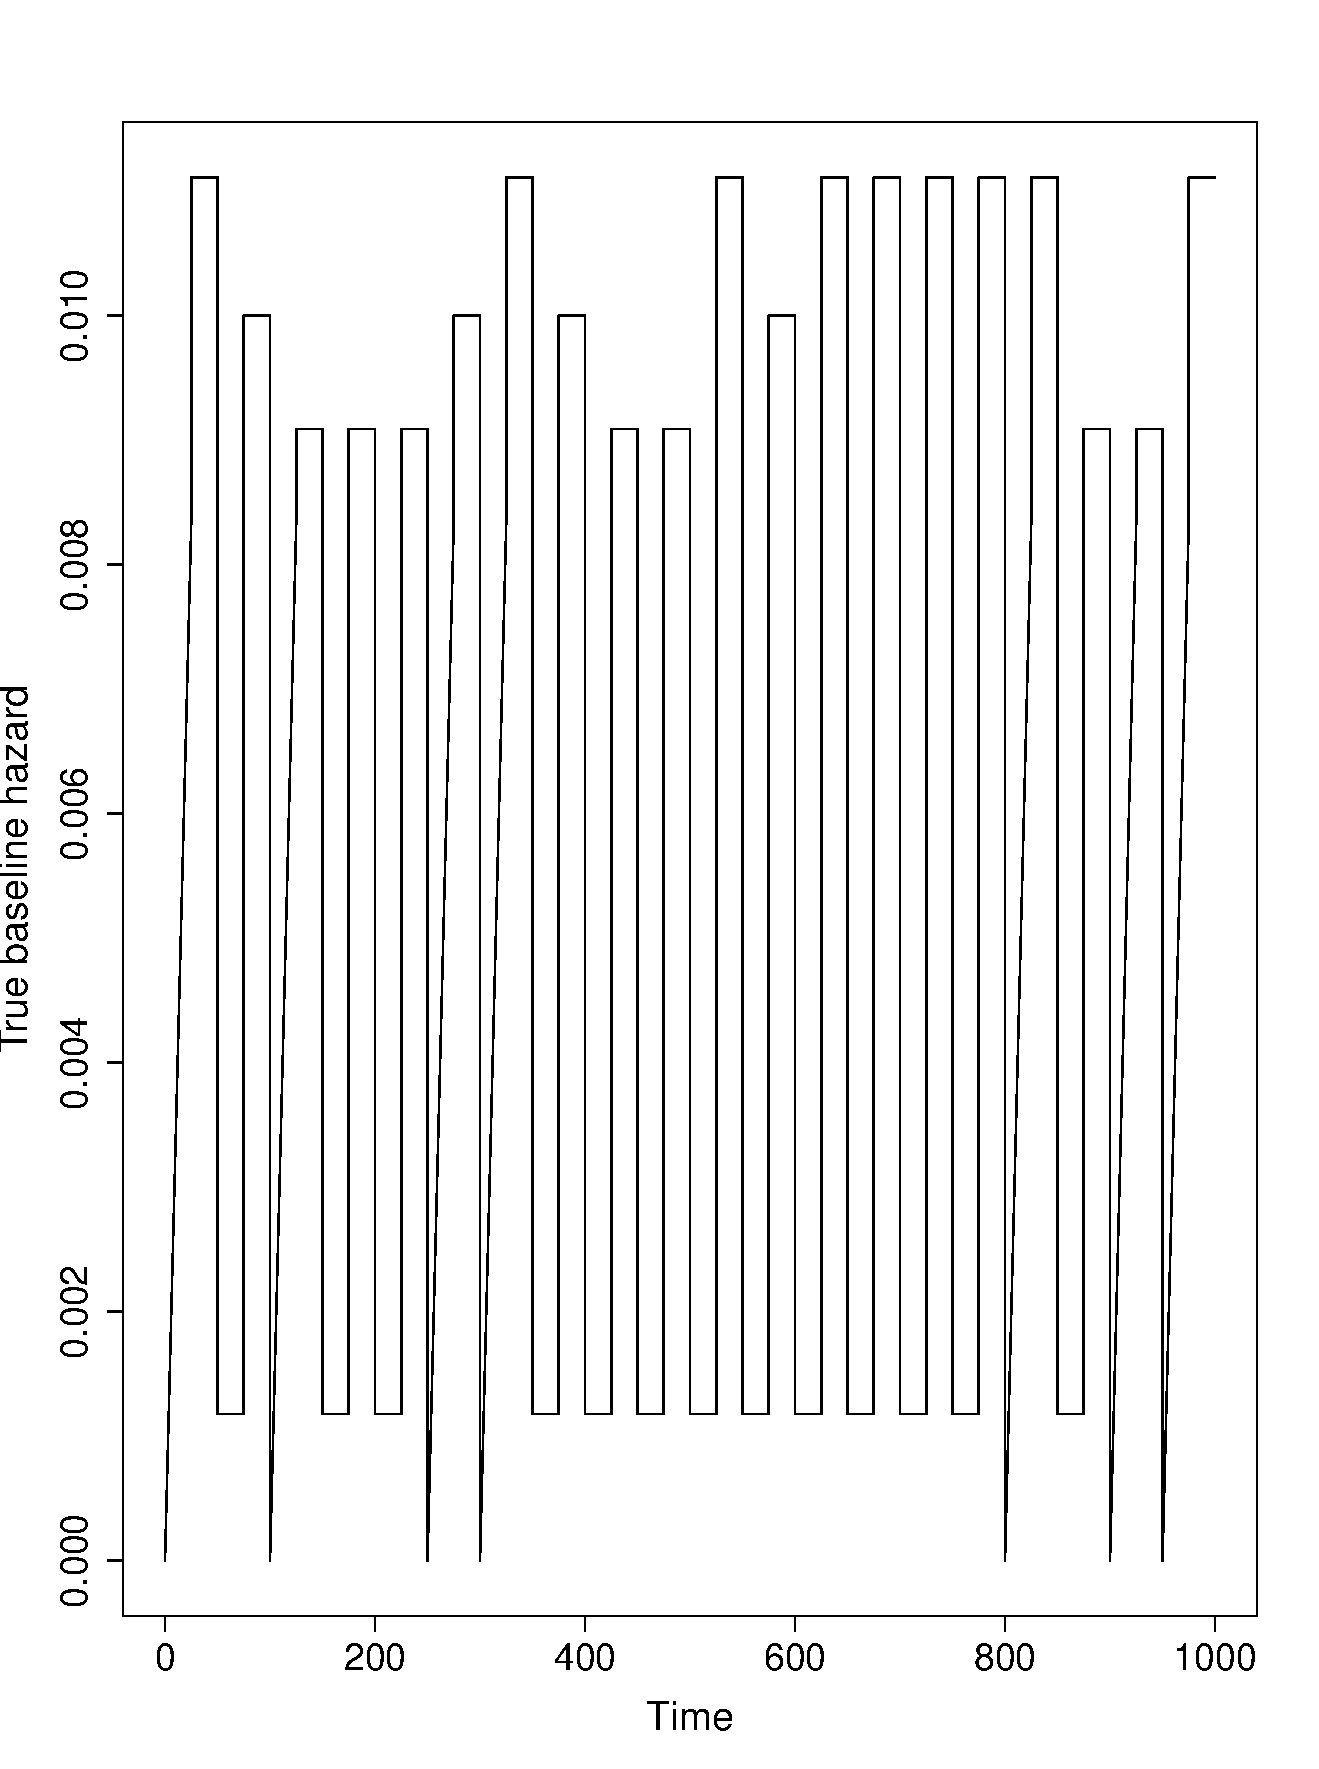
\includegraphics[width=0.45\textwidth,height=3.5in]{sim_base}
}
\subcaptionbox{Posterior for variance parameter $\sigma$}{
	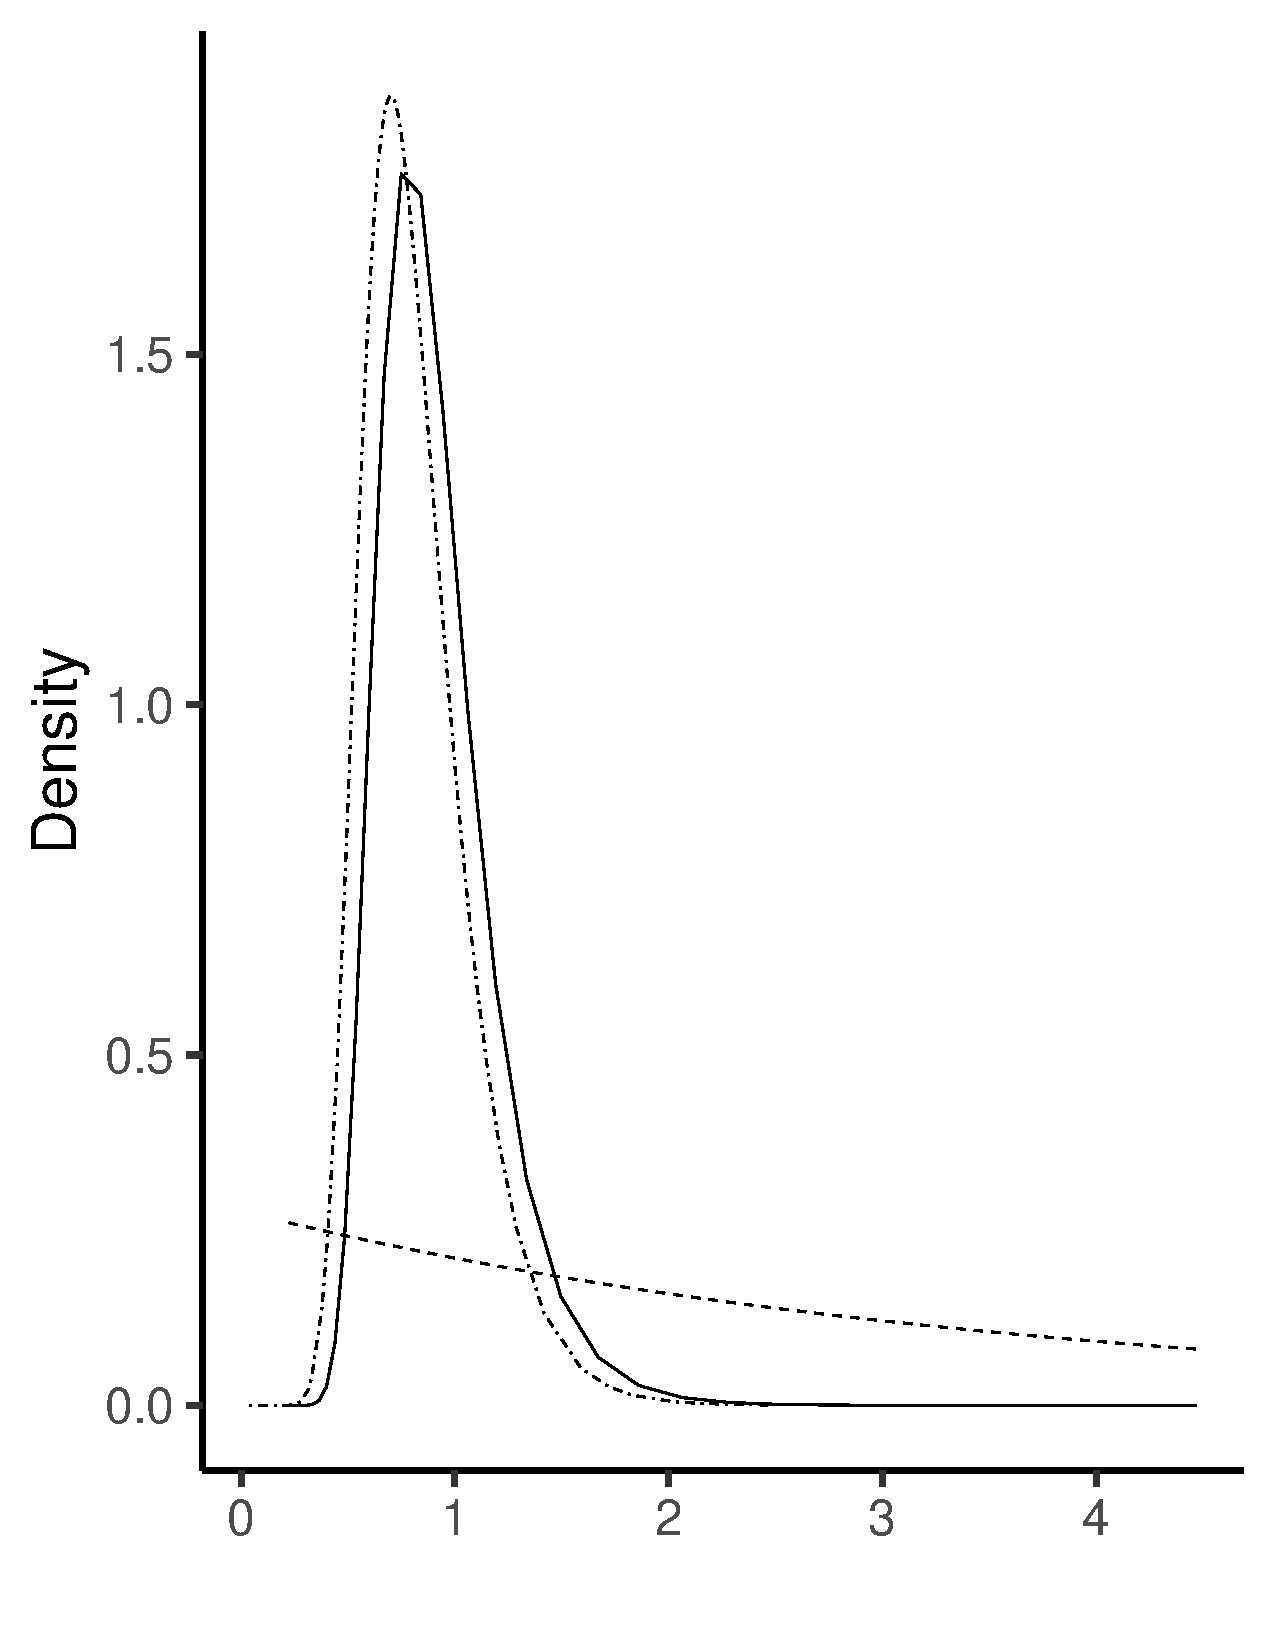
\includegraphics[width=0.45\textwidth,height=3.5in]{SmoothingSim_PosterSigma}
}
\subcaptionbox{Smoothing result}{
	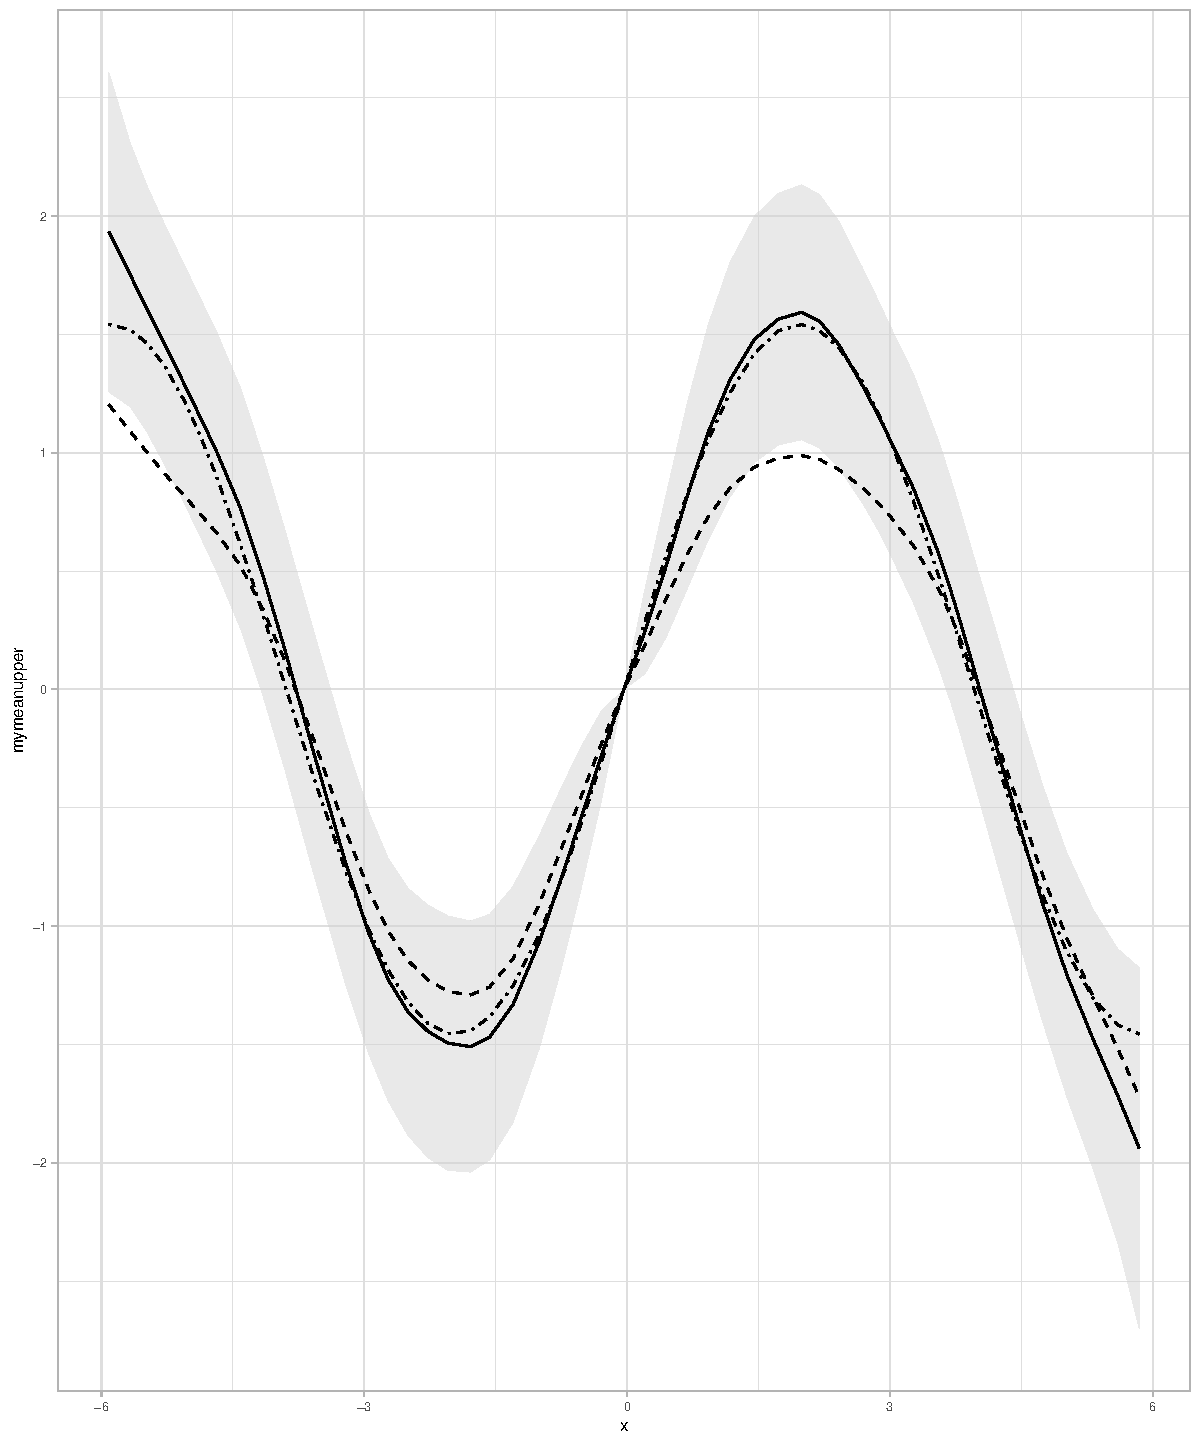
\includegraphics[width=0.45\textwidth,height=3.5in]{SmoothingSim_FinalPlot}
}

\caption{Baseline hazard function in this simulation (top left panel) Posterior Estimation for variance parameter (---) and its prior (- - -)  (top right panels). Bottom panel shows the true risk function (- $\cdot$ -), posterior mean (---) and $95\%$ credible interval using proposed method, posterior mean using INLA (- - -).}
\label{fig:simulation}
\end{figure}


Based on the Figures \ref{fig:simulation} and at above, it can be seen that our method captures the true risk function very well and outperforms INLA, which has to assume the baseline hazard function in \ref{fig:simulation} is smooth. The posterior distribution for $\sigma$ from our method is shown in the figure above as well.

\subsection{Leukaemia Data}

In this example, we will use our proposed methodology to analyse the Leukaemia data set \citet{inlacoxph} did using INLA, and compare these results with the frequentist method GAM. The data set contains 1043 of adult leukaemia patients' information with around 16 percent of them being right-censored. 

For our implementation, we are interested in quantifying the relationship between survival rate of leukaemia patients with the age of the patient ($\text{age}$), the count of white blood cells at diagnosis ($\text{wbc}$), the Townsend deprivation index ($\text{tpi}$) and patient's sex ($\text{sex}$). The effects of $\text{sex}$, $\text{age}$ and $\text{wbc}$ were modelled linearly, and the $\text{tpi}$ was modelled as a semi-parametric smoothing effect. The smoothing variable $\text{tpi}$ was discretized into 50 equally spaced bins. Our methodology does not require the smoothness assumption on the baseline hazard function nor a specification of it.

We set the prior distributions for all the linear effects $\beta$ as $\beta \stackrel{iid}{\sim} \text{N}(0, 0.05^{-1})$, and for the second order random walk of $\Gamma_1 = \{\Gamma_{1,1}, ..., \Gamma_{1,50}\}$ as $\Gamma \sim \text{RW}_2(\sigma^2)$ where a PC prior is put on $\sigma$ such that $\text{P}(\sigma > 3) = 0.5$ \citep{pcprior}. Therefore, the final dimension of W in this example will be 1094. We fit this model using both INLA and our proposed methodology, and then their smoothing results are compared with the result of GAM. For INLA's implementation, it has to assume the smoothness of the baseline hazard and then model it semi-parametrically using random walk model. 

\begin{figure}[ht]
\centering
\subcaptionbox{Posterior for variance parameter $\sigma$}{
	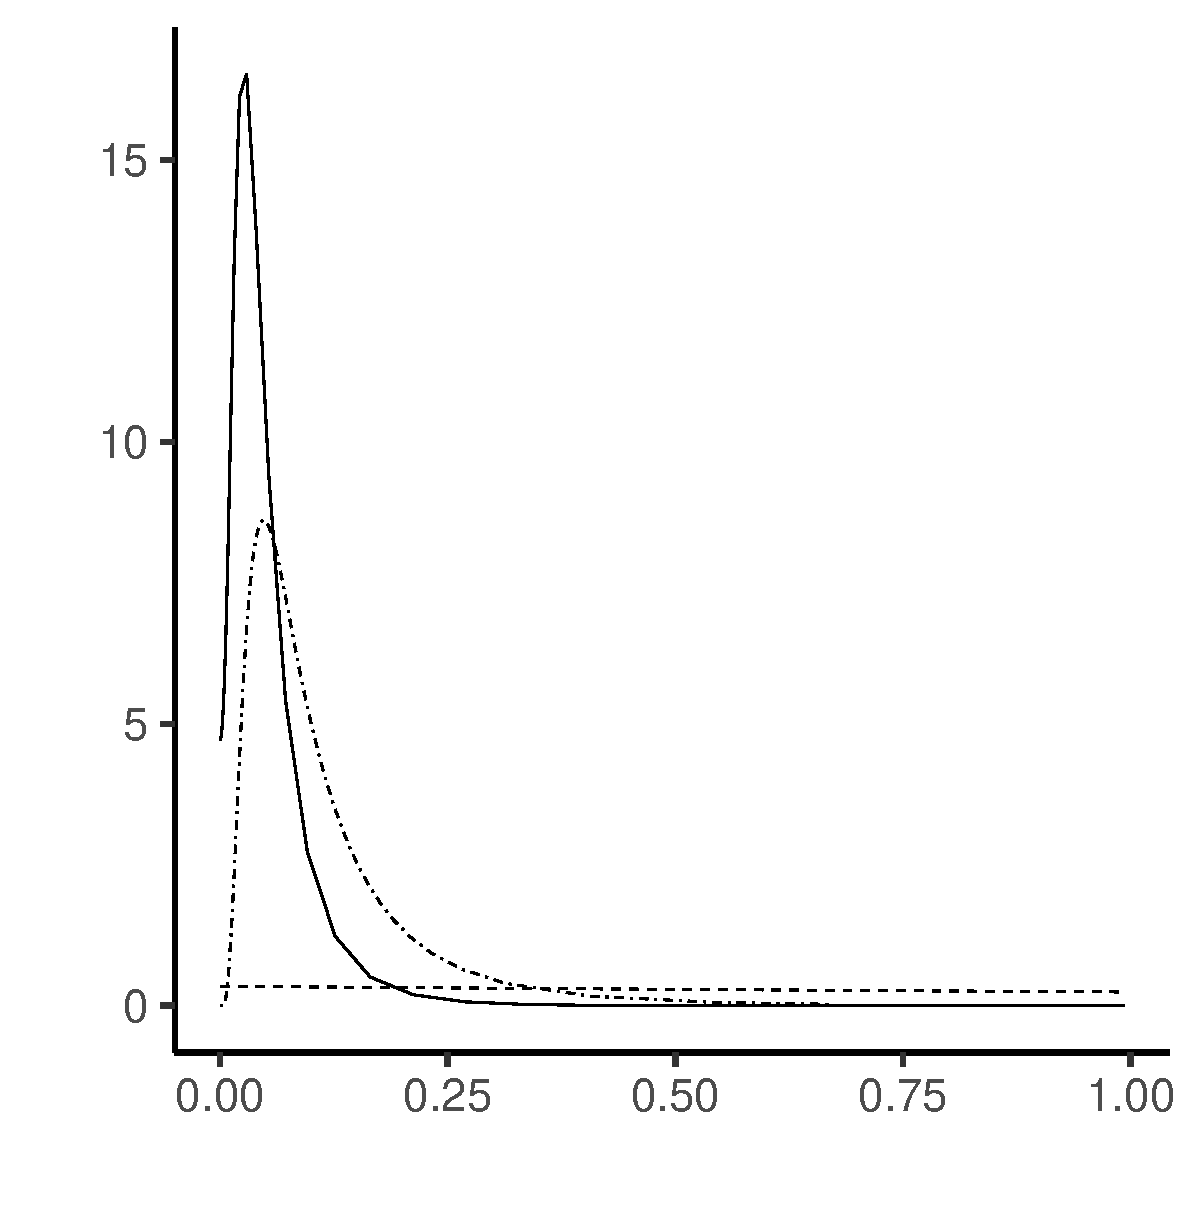
\includegraphics[width=0.45\textwidth,height=3.5in]{Leuk_PosterSigma}
}
\subcaptionbox{Smoothing result}{
	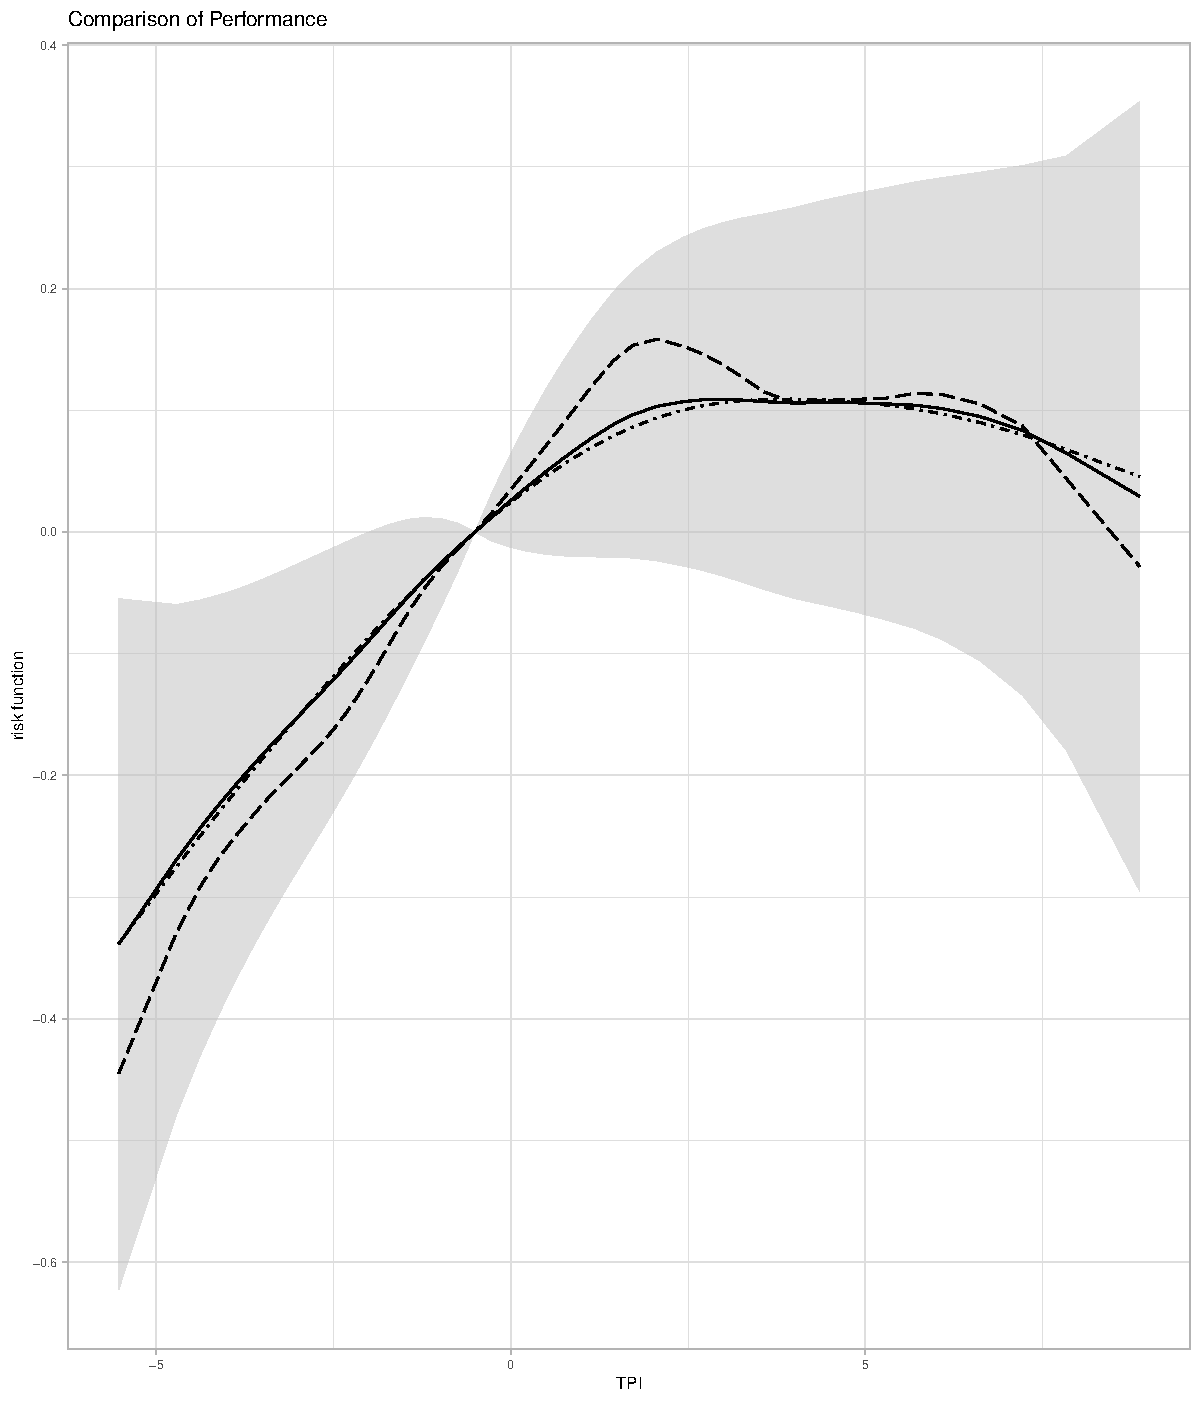
\includegraphics[width=0.45\textwidth,height=3.5in]{leuk_FinalPlot}
}

\caption{Posterior Estimation for variance parameter (---) and its prior (- - -)  (left panel). Right panel shows the posterior mean (---) and $95\%$ credible interval using proposed method, posterior mean using INLA (- - -) and the smoothing result of GAM (- $\cdot$ -).}
\label{fig:leuk}
\end{figure}


Figure \ref{fig:leuk} shows the comparison result of these three methods. It can be seen that the smoothing result given by our method is very similar to the one given by GAM, while the result given by INLA seems comparatively more wiggly. This lack of smoothness may be caused by the inappropriate assumption that INLA put on the form of this baseline hazard function, and in this case it becomes a reason to choose our method or GAM which use the partial likelihood function and hence do not require the specification of the baseline hazard function.

Figure \ref{fig:leuk} shows the posterior distribution of variance parameter given by our algorithm. Based on this plot, it seems like $\sigma$'s value is likely to be very close to zero, which indicates high smoothness on the smoothing function $\Gamma$. This type of model-based quantification of smoothness is a reason to choose Bayesian method over frequentist method such as GAM.


\subsection{Kidney Catheter Data}

In this example, we implement our proposed methodology to analyse the kidney catheter data set that \citet{kidney} analysed using Cox proportional hazard model. This data set contains 76 recurrence times to infection, at the point of insertion of the catheter, for 38 kidney patients. In this data set, each kidney patient has exactly two observations, each observation from one kidney. When the catheter is removed for other reason than infections, the observation is right censored.

In our analysis, we mostly followed the procedures \citet{kidney} did in their work, and aimed to quantify the relationship between recurrence time of bladder infection with patient's age, sex and  disease types. The variable sex is coded as 1 for male and 2 for female. The four diseases types are represented by three dummy variables $\text{GN}$, $\text{AN}$ and $\text{PKD}$, with the reference group being $Other$. A patient level frailty is also added to the model, such that observations within the same patient are correlated. 

We specified the prior distributions for all the linear effect $\beta$ as $\beta \stackrel{iid}{\sim} \text{N}(0, 0.05^{-1})$ , and the prior distribution for the standard deviation of the between-subjects frailty as a PC prior such that $\text{P}(\sigma > 2) = 0.5$. As a comparison, we also implemented INLA and frequentist maximum partial likelihood method for this model. The result is summarized at the figures below.

\begin{figure}[ht]
\centering
\subcaptionbox{Estimated means of linear effects}{
	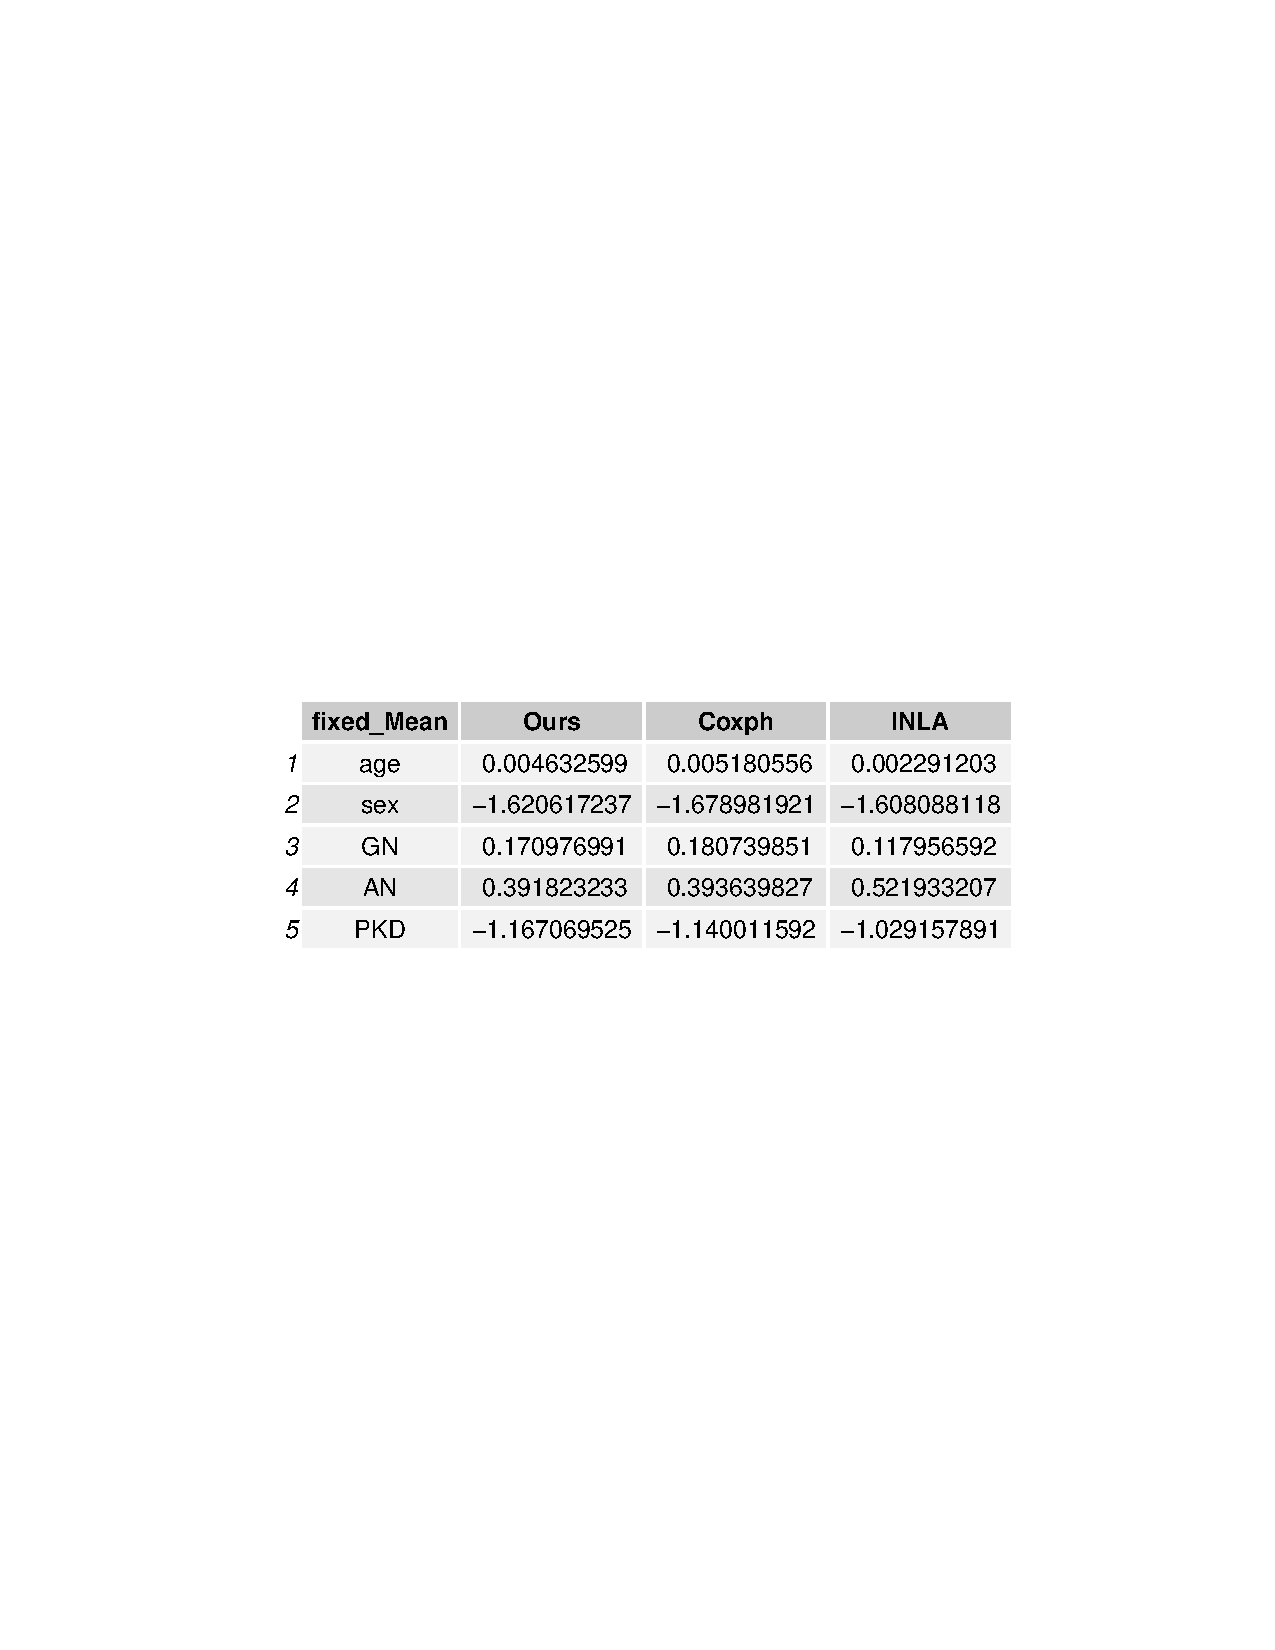
\includegraphics[width=0.75\textwidth,height=3.5in]{FixedEffectsMean}
}
\subcaptionbox{Posterior standard deviations of linear effects }{
	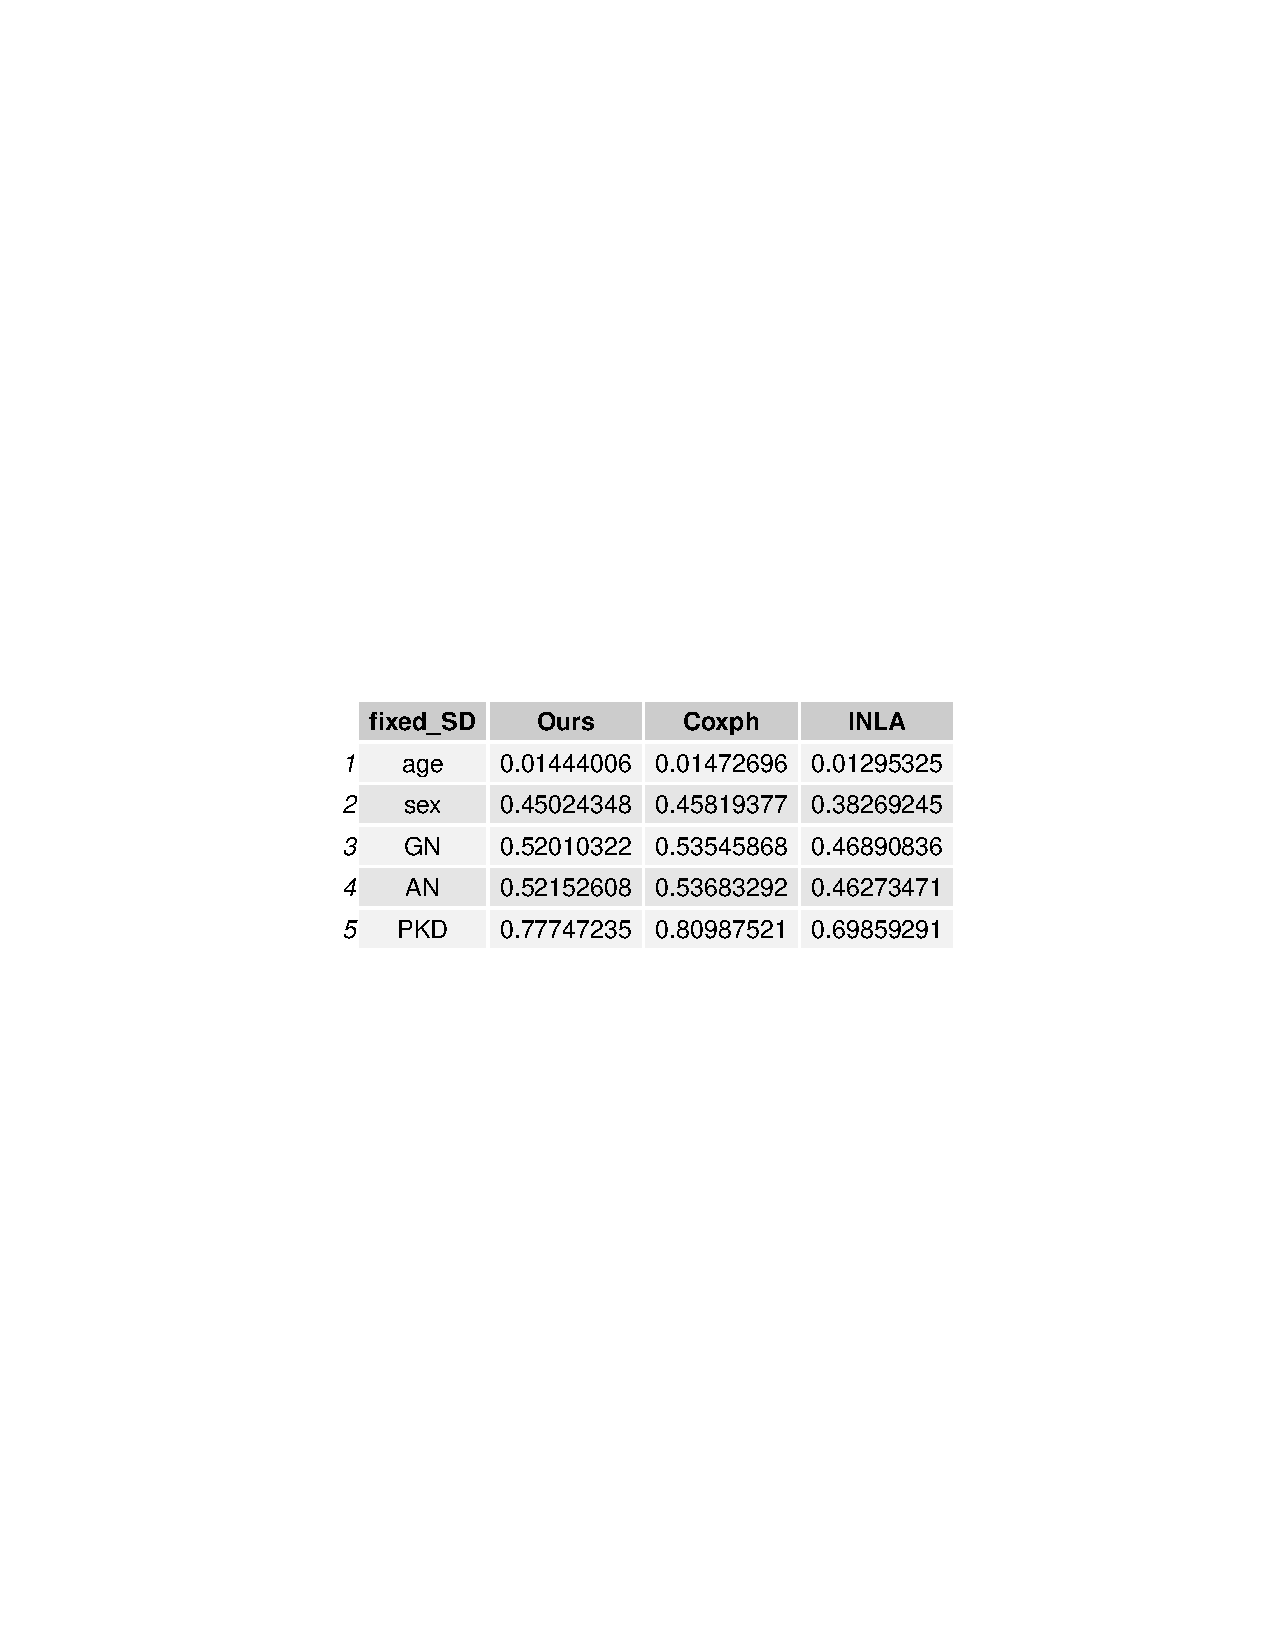
\includegraphics[width=0.75\textwidth,height=3.5in]{FixedEffectsSD}
}
\caption{Posterior Estimation and Maximum Partial likelihood Estimation for linear effects}
\label{fig:BladderLinearEff}
\end{figure}

From figure \ref{fig:BladderLinearEff}, it can be seen that for the inference of linear effects, the posterior means given by our proposed method are very similar to the frequentist's maximum partial likelihood estimates. While the posterior means given by INLA tends to be less similar to the results of the above two methods. Besides that, the posterior standard deviations of these linear effects given by our proposed methods are similar to the estimated standard errors given by maximum partial likelihood methods, but the posterior deviations given by INLA tend to be smaller.

\begin{figure}[ht]
\centering
\subcaptionbox{Posterior for the between-subject standard deviation $\sigma$}{
	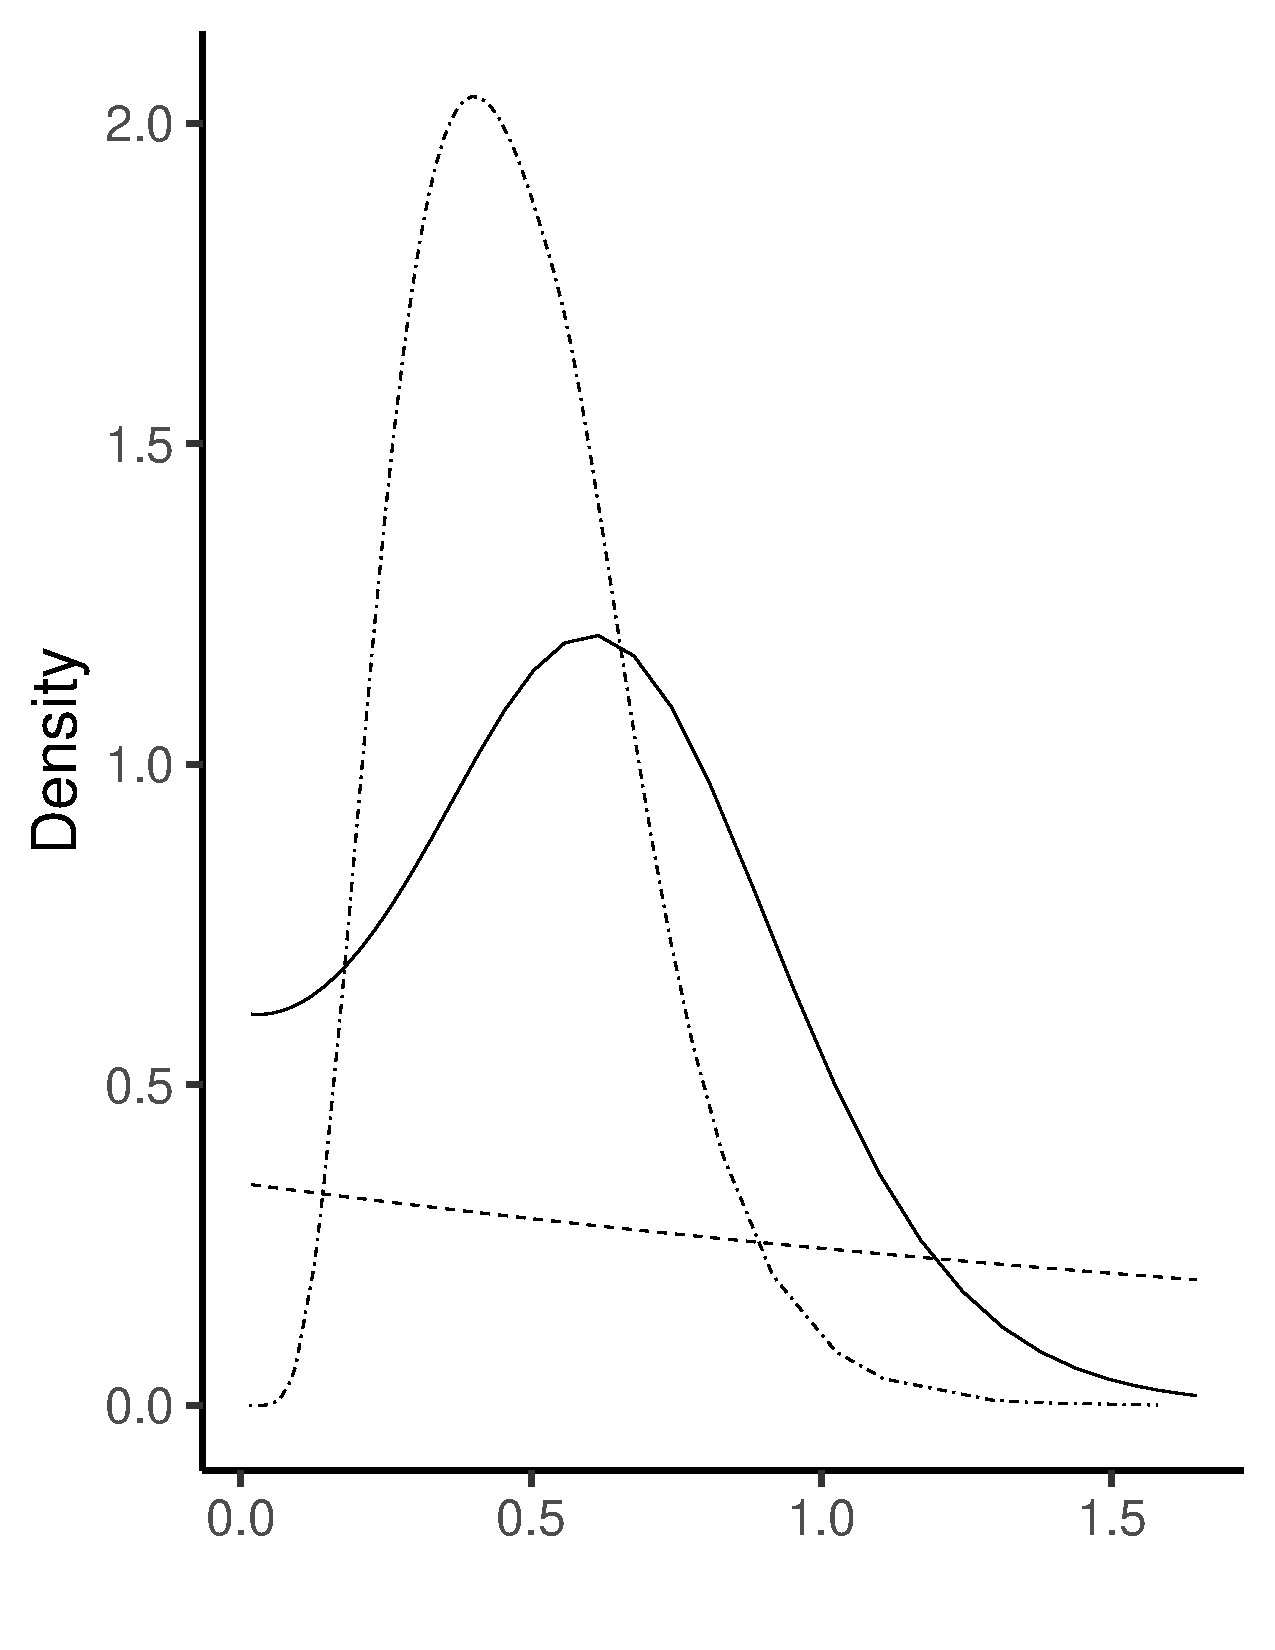
\includegraphics[width=0.45\textwidth,height=3.5in]{Kidney_PosterSigma}
}
\caption{Posterior Estimation for the between-subject standard deviation (---) and its prior (- - -)  (left panel)}
\label{fig:BetweenSubjectSD}
\end{figure}

As contrast to maximum partial likelihood method, our proposed method is able to give a model-based quantification of the between-subject standard deviation $\sigma$. The figure \ref{fig:BetweenSubjectSD} above shows the posterior distribution for the between-subject standard deviation. 



\section{Discussion}\label{sec:discussion}

The novel methodology we proposed in this paper provides a flexible way to do approximate Bayesian inference on Cox proportional hazard model with linear effects, semi-parametric smoothing effects and between-groups frailty. This methodology uses partial likelihood hence does not require the smoothness assumption on the baseline hazard function, which is assumed by INLA as it uses the full likelihood instead. It provides model-based uncertainty quantification of the smoothness parameter and between-groups standard deviation as compared to the bootstrapping method used by frequentist method such as GAM. We have demonstrated its accuracy over alternative approaches through the simulation study, and illustrated its model-based uncertainty quantification through the simulation study and the two real data analysis. As long as the inference on baseline hazard function is of secondary interest, our proposed method will be an appealing option to adopt for the analysis of small to median-size data set.

One limitation of our proposed methodology would be its unscalability to data set with massive size. Since the Hessian matrix in our methodology is fully dense and its number of entries increases quadratically with the sample size, the memory cost will become too heavy for our proposed method to be feasible if the sample size is very large. We avoid the computation of this Hessian matrix during the optimization step by implementing a quasi-Newton method that approximates the true Hessian matrix using update of rank 1, but the true Hessian matrix is still required to be evaluated at the maximum to obtain the posterior inferential result. 

The framework of this proposed methodology can be easily extended to fit more complex model, by modifying the covariance structure of the covariate with semi-parametric effect. For example, adding a covariate with spatially correlated covariance structure such as simultaneously autoregressive model (SAR) can allow the inclusion of spatial effect into the Cox PH model \citep{Spatial}. We will leave these possible extensions to future works.

\newpage

\bibliographystyle{biom}
\bibliography{myrefs}



\end{document}